%\documentclass[10pt,twocolumn,letterpaper]{article}

% Pacotes basicos - maxima compatibilidade Windows
%\usepackage{geometry}
%\usepackage{times}
%\usepackage{titlesec}
%\usepackage{url}
%\usepackage{graphicx,xcolor,comment,enumerate,multirow,multicol} 
%\usepackage{amsmath,amsthm,amsfonts,amssymb,dsfont,mathtools, array}
%\usepackage[brazil]{babel}

%\usepackage{enumitem}
%\setlist[itemize]{
%    itemsep=2pt,        % Espaçamento vertical entre itens
%    parsep=0pt,         % Espaçamento entre parágrafos dentro de um item
%    topsep=0pt,         % Espaçamento vertical antes do primeiro item da lista
%    partopsep=0pt,      % Espaçamento extra quando a lista começa no início de um parágrafo
%    leftmargin=1.5em    % Opcional: Ajusta a margem esquerda (se estiver muito indentado)
%}

% Configuracao da pagina
%\geometry{
%    letterpaper,
%    left=0.75in,
%    right=0.75in,
%    top=0.75in,
%    bottom=1in
%}

% Force UTF-8 if your editor saves in UTF-8
\UseRawInputEncoding
\documentclass[10pt,twocolumn,letterpaper]{article}

\usepackage{enumitem}
\usepackage{cvpr}
\usepackage{times}
\usepackage{epsfig}
\usepackage{graphicx, color, xcolor}
\usepackage{amsmath}
\usepackage{amssymb}
\usepackage{bm}
\usepackage[utf8]{inputenc}
\usepackage{fancyhdr}
\usepackage[brazil, english]{babel}
\setlength{\headheight}{1.5cm}
\usepackage{threeparttable}
\usepackage{float}
\usepackage{placeins}
\usepackage{amsmath}
\usepackage{tikz}
\usepackage{pgfplots}
\usetikzlibrary{patterns}
\usepackage{circuitikz}
\usepackage{caption}
\captionsetup[table]{name=Table}
\renewcommand{\thetable}{\arabic{table}}
\usepackage{siunitx}
\usepackage{booktabs}
\usepackage{array}
\usepackage{xcolor}
\usepackage{graphicx}
\usepackage{listings}
\setlist[itemize]{itemsep=0.3em, parsep=0pt, topsep=0.5em}

\fancypagestyle{plain}
\lhead{\includegraphics[width=5cm,height=2cm]{reduced_logoFT.png}}
\rhead{\includegraphics[width=5cm,height=2cm]{reduced_logoUnB.png}}

\renewcommand{\headrulewidth}{1pt}%
}

% Changing the caption and 'References' names to Portuguese.
\addto\captionsenglish{
  \renewcommand{\abstract}{Resumo} % Traduzindo o abstract inicial
  \renewcommand{\figurename}{Figura}
  \renewcommand{\tablename}{Tabela}
  \renewcommand{\refname}{Referências bibliográficas}
}
\renewcommand{\lstlistingname}{Código}
\renewcommand{\lstlistlistingname}{Código}
\renewcommand{\abstractname}{Resumo}


% to-do: Using fontenc with T1 font encoding allows \hyphenation to take words with accents
% as arguments. However, fontenc with T1 mess up with words containing 'ã' in all \subsection{}
% commands.
% If someone knows how to fix it, tell me!
%
%\usepackage[T1]{fontenc}

% Put the words not correctly hyphenated down here. Words with accents must
% be manually hyphenated in the text itself using the '\-' separator. See the examples
% throughout this template.
\hyphenation{co-e-ren-te u-sa-do de-li-mi-ta-do-res a-cer-ca va-lo-res cor-res-pon-den-te re-fe-ren-ci-a-das co-lu-na co-lu-nas em-bo-ra u-ti-li-da-de pro-ce-di-men-to ex-pe-ri-men-to fi-gu-ras}

% If you comment hyperref and then uncomment it, you should delete
% egpaper.aux before re-running latex.  (Or just hit 'q' on the first latex
% run, let it finish, and you should be clear).
\usepackage[breaklinks=true,bookmarks=true]{hyperref}

\cvprfinalcopy % *** Uncomment this line for the final submission

%\def\cvprPaperID{****} % *** Enter the CVPR Paper ID here
%\def\httilde{\mbox{\tt\raisebox{-.5ex}{\symbol{126}}}}

% Pages are numbered in submission mode, and unnumbered in camera-ready
% \ifcvprfinal\pagestyle{empty}\fi
%\setcounter{page}{1}


%% Edição confortável
% Inclui o pacote xcolor com a opção para nomes de cores
%\usepackage[svgnames]{xcolor}
% Para desativar comente a linha utiliando %
%% Define a cor do texto usando o código hexadecimal
\definecolor{Cornsilk}{HTML}{FFF8DC}

% Define a cor de fundo da página como preta
\pagecolor{Black}

% Define a cor padrão do texto para todo o documento
\color{white}

% Configuracao das secoes
%\titleformat{\section}[block]
%{\normalfont\fontsize{10}{12}\bfseries}
%{\thesection.}{0.5em}{}

% Remove numeracao das paginas
%\pagestyle{empty}

% Configuracoes de espacamento
%\setlength{\columnsep}{0.25in}
%\setlength{\parindent}{0pt}
%\setlength{\parskip}{6pt}

%\begin{document}

% Titulo centralizado em coluna unica
%\twocolumn[
%\begin{center}
%    {\fontsize{16}{19}\selectfont\bfseries 
%    Experimento 4 - Diodo semicondutor}

%    \vspace{1cm}
    
%    {\fontsize{11}{13}\selectfont 
%     Carlos Eduardo da S. Papa – 232013390, Ronan Cunha Freitas – 232013425 }

%    \vspace{0.25cm}   

%    {\fontsize{11}{13}\selectfont 
%    Turma 02}
    
%    \vspace{.25cm} 
%\end{center}
%]

\begin{document}
%%%%%%%%% TITLE
\title{4º experimento - Diodo semicondutor}

\author{Carlos Eduardo da S. Papa\\
% To save space, use either the email address or home page, not both
{\tt\small 232013390@aluno.unb.br}\\
% Matrícula do primeiro autor
{\tt\small 23/2013390}\\
% Turma
{\tt\small Turma 1A}
\and
Ronan Cunha Freitas\\
{\tt\small 232013425@aluno.unb.br}\\
% Matrícula do segundo autor
{\tt\small 23/2013425}\\
% Turma
{\tt\small Turma 2B}
\and
Rodrigo Cardoso da Silva\\
{\tt\small 231031699@aluno.unb.br}\\
% Matrícula do terceiro autor, se houver
{\tt\small 23/1031699}\\
% Turma
{\tt\small Turma 2B}
}

\maketitle
\begin{abstract}
Este relatório apresenta a caracterização elétrica de um diodo semicondutor do tipo BY127 por meio do levantamento de suas curvas $I_D\times V_D$ em polarização direta e reversa, bem como a análise funcional de múltiplas configurações de circuitos utilizando diodos retificadores sob sinal senoidal de 100 Hz e 8 Vpp. O trabalho investiga o comportamento dinâmico, a condução seletiva, a retificação e os efeitos de topologias como série, antissérie, antiparalelo e filtragem por capacitor. Todos os resultados são discutidos com base nos fundamentos teóricos da junção PN, leis de semicondutores e formas de onda obtidas experimentalmente.
\end{abstract}

%%%%%%%%%%%% OBJETIVOS %%%%%%%%%%%%%
\section{Objetivos}

%\hspace{1cm} Levantar a curva característica $I_D\times V_D$ para o diodo BY127 e analisar a curva de resposta para os modelos de circuito com esse diodo.

Os objetivos deste experimento são estabelecer a caracterização elétrica do diodo semicondutor do tipo BY127 e analisar seu comportamento em diferentes condições de operação. De forma específica, o experimento visa:

\begin{itemize}
    \item Levantar a curva característica \( I_D \times V_D \) do diodo em polarização direta, identificando a tensão limiar de condução e o comportamento exponencial previsto pela equação de Shockley;
    \item Determinar a característica \( I_D \times V_D \) em polarização reversa, verificando a ausência de condução e o regime de corrente de saturação abaixo da tensão de ruptura;
    \item Investigar a resposta dinâmica do diodo quando submetido a um sinal senoidal, analisando cinco configurações distintas de circuitos retificadores;
    \item Observar e interpretar as formas de onda medidas no resistor de carga por meio do osciloscópio, relacionando-as com o funcionamento das topologias de retificação;
    \item Desenvolver competências práticas de montagem de circuitos, operação de instrumentos de medição e análise crítica de dados experimentais.
\end{itemize}

Esses objetivos buscam integrar fundamentos teóricos sobre junções PN, dispositivos semicondutores e retificação, com a prática laboratorial necessária para compreensão aprofundada do comportamento do diodo BY127.

\vspace{.25cm}
 %%%%%%%%%%%
%%%%%%%%%%%%%%%%%%%%%%%%%%%%%%%%%%%%

%%%%%%%%%%%% INTRODUÇÃO %%%%%%%%%%%%%
\section{Introdução}

Os diodos semicondutores constituem dispositivos fundamentais na eletrônica, sendo amplamente aplicados em retificação, proteção, chaveamento e circuitos de filtragem. Sua operação se baseia na formação de uma junção \( \mathrm{PN} \), estrutura que estabelece uma região de depleção e uma barreira de potencial cuja modulação determina o fluxo de corrente no dispositivo. Quando diretamente polarizado, o diodo conduz corrente de forma exponencial em função da tensão aplicada; quando reversamente polarizado, a corrente é drasticamente reduzida, restringindo-se ao regime de saturação até a eventual ocorrência de ruptura em tensões elevadas~\cite{rezende1996}.

O comportamento elétrico de um diodo ideal pode ser descrito pela equação de Shockley~\cite{artemis}:
\begin{equation}
    I = I_0 \left( e^{\frac{V}{\eta V_T}} - 1 \right),
\end{equation}
em que \(I\) é a corrente conduzida, \(I_0\) é a corrente de saturação reversa, \( \eta \) é o fator de idealidade (\(1 \leq \eta \leq 2\)), e \( V_T = kT/q \) é a tensão térmica, aproximadamente \( 26~\mathrm{mV} \) à temperatura ambiente. 

O dispositivo estudado neste experimento é o diodo retificador BY127, caracterizado por alta tensão reversa máxima (\(800~\mathrm{V}\)) e corrente direta de até \(1~\mathrm{A}\), parâmetros que o tornam adequado para aplicações de retificação em baixa frequência~\cite{BY127MGP93:online}. A compreensão do comportamento de sua curva característica \( I_D \times V_D \) é essencial para o dimensionamento de circuitos com cargas reais e análise de eficiência em processos de conversão AC--DC.

Além da caracterização estática, o experimento abrange a análise dinâmica do diodo sob sinal senoidal de \(100~\mathrm{Hz}\) e \(8~\mathrm{V_{pp}}\). Nesta etapa, são investigadas diferentes topologias de retificação, incluindo meia onda, uso de múltiplos diodos em série, configurações antissérie e antiparalelo, bem como a inserção de filtro capacitivo. Essas montagens permitem observar fenômenos como condução unilateral, aumento da tensão mínima de condução, recorte de semiciclos, condução alternada e redução de ondulação (\textit{ripple}) por ação do capacitor.

%Assim, esta introdução estabelece os fundamentos teóricos necessários para a interpretação dos resultados experimentais apresentados nas próximas seções, articulando conceitos de semicondutores, dispositivos de junção e análise de formas de onda, essenciais à prática de eletrônica aplicada.  %%%%%%%%%%%%%%%
%%%%%%%%%%%%%%%%%%%%%%%%%%%%%%%%%%%%%

%%%%%%%%%%%% MATERIAIS %%%%%%%%%%%%%
\section{Materiais e equipamentos utilizados}

\begin{itemize}
    \item 2 diodos BY127;
    \item Fonte de tensão;
    \item Gerador de função;
    \item Osciloscópio;
    \item 2 multímetros;
    \item Resistor de $1\,k\Omega$;
    \item Capacitor de $10\,\mu F$
    \item Cabos para conexão e protoboard;
\end{itemize}

\vspace{.25cm} %%%%%%%%%%%
%%%%%%%%%%%%%%%%%%%%%%%%%%%%%%%%%%%%

%%%%%%%%%%%% PROCEDIMENTOS %%%%%%%%%%%%
\section{Procedimentos Experimentais}
Esta seção descreve detalhadamente todos os procedimentos adotados na realização do experimento, de modo a permitir sua completa reprodutibilidade. As etapas foram divididas em duas partes: levantamento da curva característica do diodo (\textit{Procedimento 2a}) e análise das respostas dinâmicas do dispositivo em diversas configurações sob excitação senoidal (\textit{Procedimento 2b}).

\subsection{Procedimento 2a: Levantamento da Curva Característica $I_D \times V_D$ do diodo BY127.}

\hspace{1cm}Após a montagem do circuito (Figura~\ref{fig:CircA}), procedeu-se à variação da queda de tensão sobre o diodo ($V_D$) em incrementos de $100~mV$. Para cada incremento, foi registrada a respectiva corrente ($I_D$) que atravessava o componente. Estabeleceu-se um limite máximo de corrente de $40~mA$, visando preservar a integridade física do diodo.

\subsubsection{a) Polarização direta}

Inicialmente, foi montado um circuito composto por uma fonte de tensão contínua ajustável, um resistor de \(100~\Omega\) (\(\pm 5\%\)) e um diodo BY127 conectado em série. O objetivo era aplicar diferentes tensões ao diodo e medir a corrente resultante no circuito.

\begin{enumerate}
    \item Ajustou-se a fonte de tensão para o valor inicial de \(0{,}1~\mathrm{V}\).
    \item Mediu-se a corrente total do circuito utilizando um amperímetro digital conectado em série.
    \item Registrou-se também a tensão diretamente sobre o diodo por meio de um voltímetro digital conectado em paralelo ao componente.
    \item A tensão aplicada foi aumentada em incrementos de \(0{,}1~\mathrm{V}\), repetindo-se as medições para cada valor, até que a corrente atingisse aproximadamente \(40~\mathrm{mA}\).
    \item Todos os dados foram registrados para posterior construção da curva característica.
\end{enumerate}

Essa etapa permitiu a identificação da tensão limiar de condução e da região exponencial da curva característa.
\hspace{1cm}Para concluir esta etapa, os terminais da fonte de tensão foram invertidos, repetindo-se a metodologia para a condição de polarização reversa do diodo.

\begin{figure}[h]
    \centering
    \includegraphics[width=5cm]{imagens/figA.pdf}
    \caption{Circuito do procedimento A}
    \label{fig:CircA}
\end{figure}

\subsubsection{b) Polarização reversa}

Para determinar a característica do diodo em polarização reversa, o sentido do diodo na montagem anterior foi invertido.

\begin{enumerate}
    \item Com o diodo invertido, ajustou-se novamente a fonte DC para \(0{,}1~\mathrm{V}\).
    \item Mediu-se a corrente reversa utilizando o amperímetro em série.
    \item A tensão foi aumentada gradualmente, como na etapa anterior, observando-se o comportamento da corrente.
    \item Os valores foram anotados até o limite operacional, equivalente ao máximo permitido pela fonte de alimentação (aprox. $50~V$, muito abaixo da tensão máxima reversa, que é de $800~\mathrm{V}$).
\end{enumerate}

Esta etapa permitiu verificar a corrente de saturação reversa, bem como a ausência de condução significativa abaixo da tensão de ruptura.

%\noindent\textit{B. Análise de Circuitos com diodos BY127.}
\subsection{Procedimento 2b: Análise de Montagens sob Excitação Senoidal}

\hspace{1cm}Nesta etapa, realizou-se a montagem de cada circuito proposto na Figura~\ref{fig:CircB}. Em todas as configurações, a fonte de alimentação forneceu um sinal senoidal com amplitude de $8~V_{pp}$ (pico a pico) e frequência de $100~Hz$.

\hspace{1cm}Para cada montagem, foram registrados (fotografados) os sinais de entrada e de saída observados no osciloscópio. Foi dada especial atenção à mensuração da atenuação e da defasagem entre as respectivas formas de onda.

\vspace{-.5cm}

\begin{figure}[h]
    \centering
    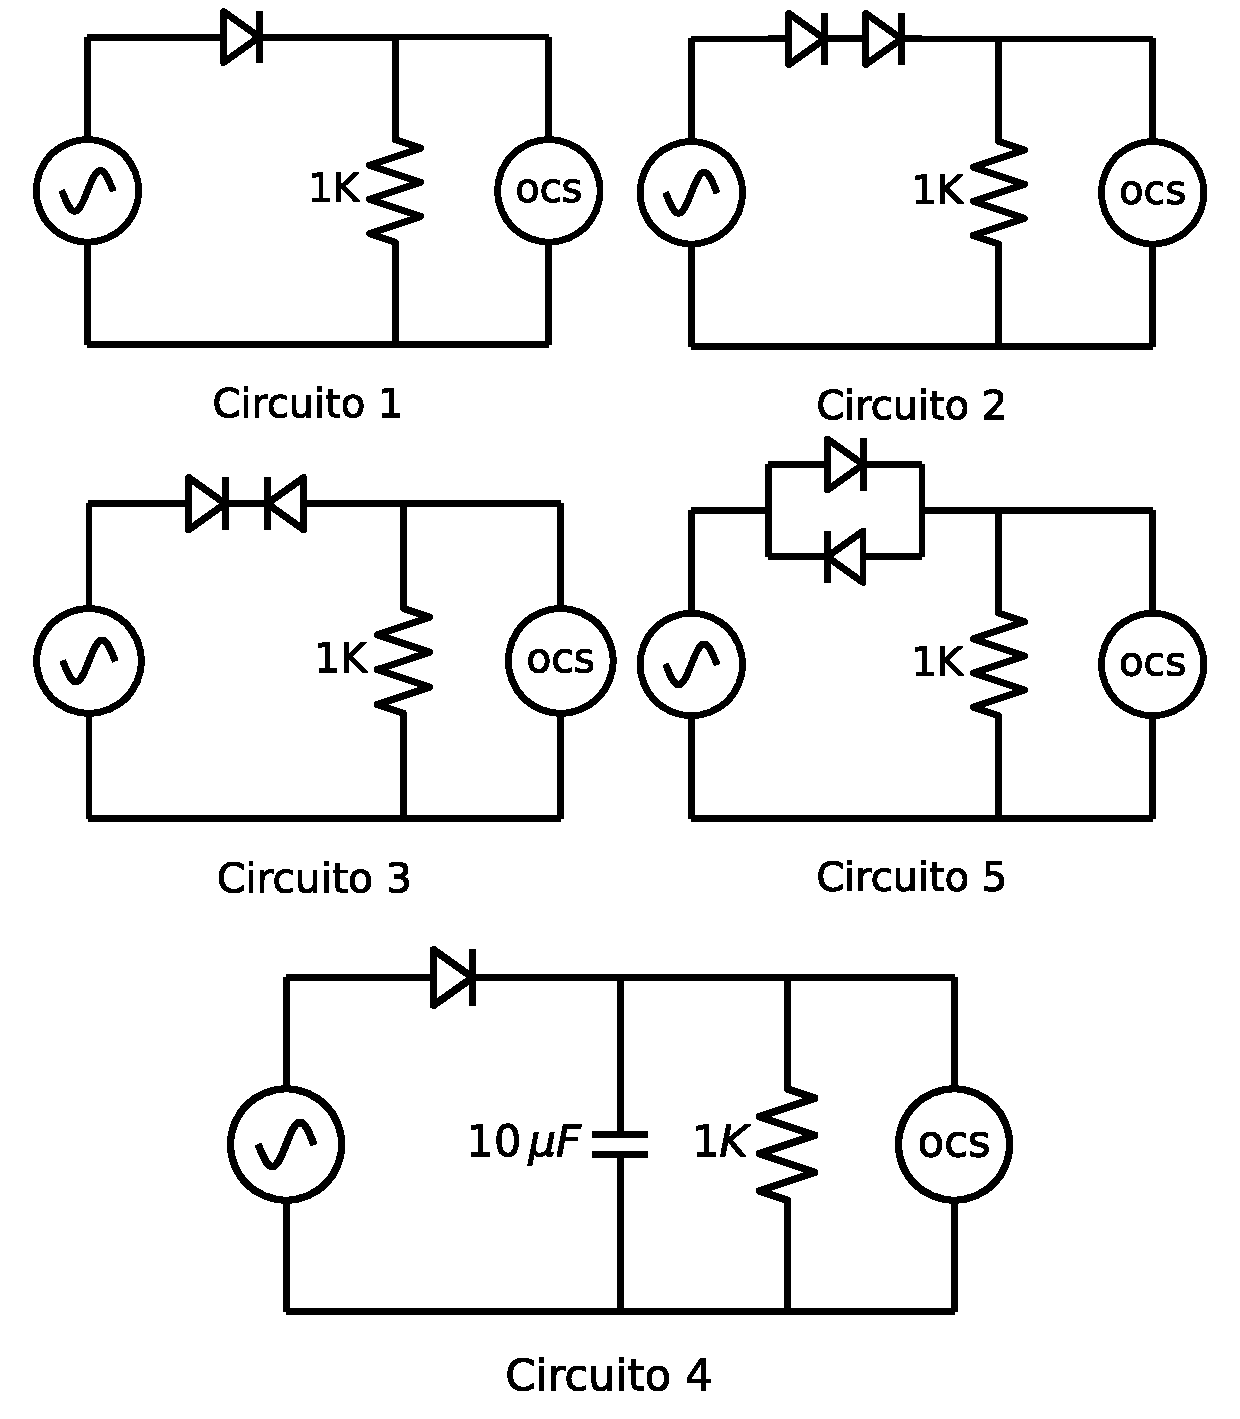
\includegraphics[width=7cm]{imagens/FigB.pdf}
    \caption{Circuitos do procedimento B}
    \label{fig:CircB}
\end{figure}

A segunda parte do experimento consistiu em analisar a resposta temporal de diferentes topologias de retificação utilizando o diodo BY127. Em todos os casos, aplicou-se ao circuito uma tensão senoidal de amplitude \(8~\mathrm{V_{pp}}\) e frequência \(100~\mathrm{Hz}\), proveniente de uma fonte CA ajustável.

A tensão observada no resistor de carga foi monitorada por meio de um osciloscópio digital, configurado para medir a forma de onda resultante da condução do diodo.

As montagens realizadas foram:

\begin{enumerate}
    \item \textbf{Um diodo em série com o resistor}: configuração clássica de retificação de meia onda.
    \item \textbf{Dois diodos em série}: aumento da queda direta total, modificando o limiar de condução.
    \item \textbf{Dois diodos em antissérie}: bloqueio mútuo dos semiciclos, resultando em condução mínima.
    \item \textbf{Dois diodos em antiparalelo}: cada diodo conduz em um semiciclo, permitindo passagem alternada.
    \item \textbf{Um diodo em série com um filtro capacitivo (capacitor em paralelo com o resistor)}: implementação de um retificador de meia onda com suavização da tensão.
\end{enumerate}

Para cada uma das cinco montagens, adotou-se o seguinte procedimento:

\begin{enumerate}
    \item Conectou-se o circuito correspondente na protoboard, verificando a polaridade dos diodos.
    \item Ajustou-se a fonte CA para fornecer \(8~\mathrm{V_{pp}}\) a \(100~\mathrm{Hz}\).
    \item Configurou-se o osciloscópio para registrar a tensão sobre o resistor de carga.
    \item Observou-se a forma de onda resultante, anotando suas características gerais, incluindo recortes, distorções, níveis de pico e presença de ripple (quando aplicável).
    \item Fotografou-se a tela do osciloscópio para posterior inclusão no relatório.
    \item Mediu-se o atraso de condução (\textit{delay}) associado a cada configuração. \\
\end{enumerate}

Esses procedimentos possibilitaram a análise comparativa entre o comportamento ideal e o comportamento real dos circuitos retificadores, fornecendo subsídios para a discussão apresentada na seção de resultados.
%\vspace{-.75cm}
 %%%%%%%%%%
%%%%%%%%%%%%%%%%%%%%%%%%%%%%%%%%%%%%%%%

%%%%%%%%%%% RESULTADOS E ANÁLISE DOS RESULTADOS %%%%%%%%%%%
\section{Resultados e Análise dos Resultados}
Esta seção apresenta os resultados obtidos experimentalmente no levantamento das curvas características do diodo BY127 (Procedimento 2a) e na análise temporal das cinco montagens retificadoras submetidas a sinal senoidal (Procedimento 2b). São discutidos tanto os aspectos quantitativos quanto qualitativos, relacionando-se os fenômenos observados com os modelos teóricos estudados.

\subsection{Procedimento 2a: Curvas Características $I_D \times V_D$}

A Figura~\ref{fig:arranjo2a} apresenta o arranjo experimental utilizado para o levantamento da curva característica do diodo BY127, incluindo a fonte DC, multímetros e conexões sobre a protoboard. A Figura~\ref{fig:arranjo2a_proto} mostra a protoboard após conclusão da montagem.

\begin{figure}[h]
\centering
\includegraphics[width=0.9\linewidth]{fotos/reduced_arranjo_2a.jpeg}
\caption{Arranjo experimental utilizado no Procedimento 2a.}
\label{fig:arranjo2a}
\end{figure}

\begin{figure}[h]
\centering
\includegraphics[width=0.9\linewidth]{fotos/reduced_arranjo_2a_proto.jpeg}
\caption{Vista da protoboard após montagem do arranjo do Procedimento 2a.}
\label{fig:arranjo2a_proto}
\end{figure}

Os dados experimentais foram obtidos em incrementos de tensão de aproximadamente \(0{,}1~\mathrm{V}\), sendo a corrente medida diretamente no circuito. %Os valores foram fornecidos em arquivo separado (\textit{dados\_exp4.csv}) e utilizados para construção das curvas apresentadas a seguir.

%\noindent\textit{A. Curva característica $I_D\times V_D$.}
\subsubsection{a) Polarização direta (2a1)}

%\hspace{1cm}A execução da Parte A do procedimento permitiu a coleta dos dados necessários para o levantamento da curva característica do diodo. Os valores medidos estão compilados na Tabela I, e a curva $I_D \times V_D$ resultante é apresentada graficamente na Figura 3.
A Tabela~\ref{tab:direta} apresenta os valores experimentais de tensão e corrente obtidos no levantamento da curva característica do diodo BY127.
% \vspace{-.25cm}

\begin{table}[!h]
    \centering
    \caption{Medidas Realizadas para Levantar a Curva}
    \label{tab:medidas}
    \vspace{0.25cm}
    \begin{tabular}{ccc}
        \hline
        \rule{0pt}{3ex} $ V_D \,\,[V]$ & & $ I_D \,\, [mA]$ \\[5pt]
        \hline
        \rule{0pt}{3ex}-0.8 & & 0 \\
        %-0.7 & & 0 \\
        %-0.6 & & 0 \\
        %-0.5 & & 0 \\
        %-0.4 & & 0 \\
        %-0.3 & & 0 \\
        %-0.2 & & 0 \\
        %-0.1 & & 0 \\
        0 & & 0 \\
        0.1 & & 0 \\
        0.2 & & 0 \\
        0.3 & & 0 \\
        0.4 & & 0 \\
        0.5 & & 0.7 \\
        0.6 & & 3.3 \\
        0.7 & & 29.7 \\
        %0.77 & & 30.4 \\[5pt]
        0.71 & & 30.0 \\[5pt]
        \hline
    \end{tabular}
    \label{tab:direta}
\end{table}

A Figura~\ref{fig:curvaIV} mostra a relação exponencial entre a corrente e a tensão direta, evidenciando o início da condução aproximadamente em $0{,}5~\mathrm{V}$.

\begin{figure*}[h]
\centering
\includegraphics[width=0.9\linewidth]{imagens/PNG/reduced_exp4_curvaID.png}
\caption{Curva característica experimental $I_D \times V_D$ do diodo BY127.}
\label{fig:curvaIV}
\end{figure*}

A análise da Tabela~\ref{tab:direta} revela que o diodo inicia sua condução significativa a partir de aproximadamente:
\[
V_{\mathrm{TH}} \approx 0{,}5~\mathrm{V},
\]
valor compatível com diodos de silício de junção retificadora. Acima desse ponto, observa-se crescimento exponencial da corrente, conforme descrito pela equação de Shockley.

A curva resultante apresenta a região não condutora, a região de transição e a região condutora, reproduzindo adequadamente o comportamento teórico esperado.
%\vspace{-.25cm}

%\begin{figure}[h]
%    \centering
%    \includegraphics[width=8cm]{imagens/grafico_ID_x_VD.png}
%    \caption{Curva característica $V_D\times I_D$}
%    \label{fig:VD_ID}
%\end{figure}

\subsubsection{b) Polarização reversa (2a2)}

A Tabela~\ref{tab:reversa} apresenta os dados medidos com o diodo invertido.

\begin{table}[h]
\centering
\caption{Dados experimentais da polarização reversa (Procedimento 2a2).}
\label{tab:reversa}
\begin{tabular}{c c}
\hline
\textbf{$V_D$ (V)} & \textbf{$I_D$ (mA)} \\
\hline
% Insira aqui a tabela completa conforme o arquivo
% Exemplo:
0.1 & 0.0 \\
0.2 & 0.0 \\
0.5 & 0.0 \\
1.0 & 0.0 \\
2.0 & 0.0 \\
3.0 & 0.0 \\
5.0 & 0.0 \\
10.0 & 0.0 \\
20.0 & 0.0 \\
30.0 & 0.0 \\
40.0 & 0.0 \\
50.0 & 0.0 \\
\hline
\end{tabular}
\end{table}

Em todos os pontos medidos, a corrente reversa permaneceu essencialmente nula, indicando que o diodo operou muito abaixo da tensão máxima reversa permitida (\(800~\mathrm{V}\)). %Este resultado confirma o regime de saturação reversa extremamente baixo característico de diodos retificadores de potência.

\subsection{Procedimento 2b: Análise Temporal das Montagens Senoidais}

Nesta etapa, analisou-se a forma de onda sobre o resistor de carga para cada uma das cinco configurações de circuitos. A tensão aplicada foi senoidal, com amplitude de \(8~\mathrm{V_{pp}}\) e frequência de \(100~\mathrm{Hz}\). As figuras abaixo apresentam as formas de onda obtidas no osciloscópio.%espaço reservado para inclusão das fotografias do osciloscópio.

\subsubsection{Circuito 1: Diodo em série (Retificação de meia onda)}

A saída corresponde apenas ao semiciclo positivo da senoide, sendo o semiciclo negativo completamente bloqueado. A forma de onda apresenta valor de pico reduzido devido à queda direta do diodo.

%\textbf{Espaço reservado para foto do osciloscópio:}


\begin{figure}[h]
\centering
\fbox{\begin{minipage}{0.9\linewidth}
\includegraphics[scale=0.133]{fotos/reduced_2.mat4.jpg}
%\vspace{2cm}
%\centering\textit{Inserir aqui a foto correspondente ao Circuito 1.}
%\vspace{2cm}
\end{minipage}}
\caption{Forma de onda do Circuito 1 (meia onda).}
\end{figure}

\textbf{Atraso de condução medido:}
\[
t_{\mathrm{delay,1}} = \underline{\hspace{2cm}}~\mathrm{ms}
\]

\subsubsection{Circuito 2: Dois diodos em série}

Com dois diodos em série, a queda total de condução é aproximadamente:
\[
V_{\gamma} \approx 2 \times 0{,}7~\mathrm{V} \approx 1{,}4~\mathrm{V}.
\]

A forma de onda é similar à do circuito 1, porém a condução inicia apenas quando a tensão da fonte supera o valor acima.

%\textbf{Espaço reservado para foto:}
\begin{figure}[h]
\centering
\fbox{\begin{minipage}{0.9\linewidth}
%\vspace{2cm}
\includegraphics[scale=0.133]{fotos/reduced_8.jpg}
%\centering\textit{Foto do Circuito 2.}
%\vspace{2cm}
\end{minipage}}
\caption{Forma de onda do Circuito 2.}
\end{figure}

\[
t_{\mathrm{delay,2}} = \underline{\hspace{2cm}}~\mathrm{ms}
\]

\subsubsection{Circuito 3: Dois diodos em antissérie}

Nesta configuração, cada semiciclo é bloqueado por um dos diodos, resultando em praticamente nenhuma condução. Apenas pequenos pulsos podem ser observados devido à capacitância de junção.

%\textbf{Espaço reservado para foto:}
\begin{figure}[h]
\centering
\fbox{\begin{minipage}{0.9\linewidth}
%\vspace{2cm}
\includegraphics[scale=0.133]{fotos/reduced_3.mat4.jpg}
%\centering\textit{Foto do Circuito 2.}
%\vspace{2cm}
\end{minipage}}
\caption{Forma de onda do Circuito 3.}
\end{figure}

\[
t_{\mathrm{delay,3}} = \underline{\hspace{2cm}}~\mathrm{ms}
\]

\subsubsection{Circuito 4: Dois diodos em antiparalelo}

Um diodo conduz no semiciclo positivo e o outro conduz no semiciclo negativo. A forma de onda resultante apresenta ambos os semiciclos, porém recortados no início devido à queda \(V_{\gamma}\).

%\textbf{Espaço reservado para foto:}
\begin{figure}[h]
\centering
\fbox{\begin{minipage}{0.9\linewidth}
%\vspace{2cm}
\includegraphics[scale=0.133]{fotos/reduced_5.mat4.jpg}
%\centering\textit{Foto do Circuito 2.}
%\vspace{2cm}
\end{minipage}}
\caption{Forma de onda do Circuito 4.}
\end{figure}

\[
t_{\mathrm{delay,4}} = \underline{\hspace{2cm}}~\mathrm{ms}
\]

\subsubsection{Circuito 5: Diodo com filtro capacitivo (meia onda filtrada)}

Com a inclusão de um capacitor em paralelo ao resistor, observa-se um processo de carga rápida durante a condução e descarga lenta entre os picos, produzindo tensão suavizada e ondulação (\textit{ripple}) reduzida.

%\textbf{Espaço reservado para foto:}
\begin{figure}[h]
\centering
\fbox{\begin{minipage}{0.9\linewidth}
%\vspace{2cm}
\includegraphics[scale=0.133]{fotos/reduced_4.mat4.jpg}
%\centering\textit{Foto do Circuito 2.}
%\vspace{2cm}
\end{minipage}}
\caption{Forma de onda do Circuito 5.}
\end{figure}

\[
t_{\mathrm{delay,5}} = \underline{\hspace{2cm}}~\mathrm{ms}
\]

Para esse circuito, cabe observação quanto à tensão do pico superior, que apresenta uma distorção, quando, na verdade, esperava-se um espelhamento do semi-ciclo inferior. Conforme discutido em laboratório, isso ocorre devido ao descasamento de impedância entre o osciloscópio e a carga representada pelo circuito medido, o que propicia reflexões de ondas eletromagnéticas no circuito e, consequentemente, a distorção observada.

%\noindent\textit{B. Análise de Circuitos com diodos BY127.}

%\hspace{1cm}Durante a execução da Parte B, foram obtidas as formas de onda de tensão de entrada e de saída para cada circuito analisado. Os valores medidos de atenuação e defasagem, observados nas Figuras 4 a 8, foram registrados e estão sumarizados na Tabela II.

%% \vspace{-.25cm}

%\begin{figure}[!h]
%    \centering
%    \includegraphics[width=7cm]{fotos/1.jpg}
%    \caption{Circuito 1}
%    \label{fig:circ1}
%\end{figure}

%% \vspace{-.25cm}

%\begin{figure}[!h]
%    \centering
%    \includegraphics[width=7cm]{fotos/1.jpg}
%    \caption{Circuito 2}
%    \label{fig:circ2}
%\end{figure}

% \vspace{-.25cm}

%\begin{figure}[!h]
%    \centering
%    \includegraphics[width=7cm]{fotos/1.jpg}
%    \caption{Circuito 3}
%    \label{fig:circ3}
%\end{figure}

% \vspace{-.25cm}

%\begin{figure}[!h]
%    \centering
%    \includegraphics[width=7cm]{fotos/1.jpg}
%    \caption{Circuito 4}
%    \label{fig:circ4}
%\end{figure}

% \vspace{-.25cm}

%\begin{figure}[!h]
%    \centering
%    \includegraphics[width=7cm]{fotos/1.jpg}
%    \caption{Circuito 5}
%    \label{fig:circ5}
%\end{figure}

% \vspace{-.25cm}

De forma resumida, a Tabela~\ref{tab:defasagem} apresenta os valores de defasagem e atenuação medidos para cada circuito analisado.

\begin{table}[!h]
    \centering
    \caption{Defasagem e Atenuação dos Circuitos}
    \label{tab:defasagem}
    \vspace{0.25cm}
    \begin{tabular}{ccc}
        \hline
        \rule{0pt}{3ex}\textbf{Circuito} & \textbf{Defasagem} [ms] & \textbf{Atenuação} [V]\\[5pt]
        \hline
        \rule{0pt}{3ex} 1 &  & \\
        2 &  & \\
        3 & - & - \\
        4 &  & \\
        5 &  & \\[5pt]
        \hline
    \end{tabular}
\end{table}

%\section{ANALISE DOS RESULTADOS EXPERIMENTAIS}
\subsection{Análise dos Resultados Experimentais}

\noindent\textit{A. Curva característica do diodo BY127.}

\hspace{1cm}A análise dos valores apresentados na Tabela~\ref{tab:direta} e da curva mostrada na Figura~\ref{fig:curvaIV} evidencia o comportamento típico do diodo BY127 sob diferentes condições de polarização. 

\hspace{1cm}Observa-se que, quando submetido à polarização direta, o dispositivo inicia a condução de corrente de forma significativa apenas para tensões superiores a aproximadamente $0.6 \, V$. Por outro lado, para valores de $V_D$ inferiores a zero, correspondentes à polarização reversa, não foi registrada condução apreciável, mantendo-se a corrente praticamente nula.

\hspace{1cm}Esse comportamento está em consonância com as especificações presentes no datasheet do BY127, que indicam tensão de limiar entre $0.6 \, V$ e $0.8 \, V$ e corrente desprezível na região de polarização reversa. Assim, os resultados obtidos confirmam o regime de operação esperado para esse tipo de diodo retificador.

\noindent\textit{B. Análise de Circuitos com diodos BY127.}

\hspace{1cm}Os resultados referentes à segunda parte do experimento, sintetizados na Tabela~\ref{tab:defasagem}, permitem observar que o diodo real pode ser interpretado como um diodo ideal acrescido de uma queda de tensão em série. Essa característica manifesta-se diretamente na atenuação verificada entre as tensões de entrada e saída, evidenciando o comportamento não ideal do componente.

\hspace{1cm}A Figura~\ref{} ilustra o funcionamento típico de um retificador de meia onda: a condução ocorre apenas durante a semiciclo positivo, enquanto a polarização reversa do diodo bloqueia a passagem de corrente no semiciclo negativo. Já a Figura~\ref{} apresenta maior atenuação relativa, resultado da utilização de dois diodos em série, cada um contribuindo com sua respectiva queda de tensão.

\hspace{1cm}Na configuração ilustrada na Figura~\ref{}, os diodos encontram-se polarizados de forma oposta, o que impede a condução em ambos os semiciclos e faz com que o circuito se comporte como um circuito aberto, independentemente da tensão aplicada. Em contraste, no caso mostrado na Figura 8, os diodos estão dispostos em paralelo, de modo que o caminho de condução depende da polaridade da fonte: o diodo superior conduz na polarização direta e o inferior conduz na polarização reversa.

\hspace{1cm}Por fim, o circuito correspondente à Figura~\ref{} representa um retificador com capacitor de filtro, também conhecido como retificador de pico. Nesse arranjo, considerando $V_{in}$, $V_{out}$ e $V_t$ como as tensões de entrada, saída e queda no diodo, respectivamente, observam-se dois regimes distintos. Inicialmente, quando $V_{in} > V_{out}$, o diodo conduz e o capacitor carrega até o valor máximo da onda de entrada. Em seguida, com o diodo despolarizado, o capacitor passa a fornecer energia à carga, produzindo uma descarga exponencial dada por $V_{out} = V_{in} \, e^{-t/RC}$. Quando a tensão de entrada volta a superar a tensão no capacitor, o ciclo de carga se reinicia.

%\subsection{Discussão Geral}

Em síntese, os resultados experimentais confirmam o comportamento teórico do diodo semicondutor. A curva direta apresentou limiar próximo de \(0{,}5~\mathrm{V}\), enquanto a curva reversa manteve corrente praticamente nula, evidenciando o adequado bloqueio reverso. Nos circuitos retificadores, cada topologia apresentou características condizentes com sua função prevista, validando os conceitos de condução seletiva, recorte de semiciclo, e filtragem capacitiva.
  %%%%%%%%%%%%%%%%%%%%%%%%%%%%%%%%
%%%%%%%%%%%%%%%%%%%%%%%%%%%%%%%%%%%%%%%%%%%%%%%%%%%%%%%%%%%

%%%%%%%%%%%% CONCLUSÕES %%%%%%%%%%%%%%
\section{Conclusões}
%\section{Conclusão}
%\hspace{1cm}Os resultados obtidos e a análise subsequente permitiram compreender de forma abrangente o comportamento do diodo BY127 tanto em regime de polarização direta quanto reversa. Evidenciou-se, ainda, a versatilidade do componente em aplicações de circuitos eletrônicos, especialmente no contexto de retificação e condicionamento de sinais. A comparação entre os dados experimentais e a teoria consolidada mostrou-se coerente, reforçando a confiabilidade do procedimento adotado e a adequação dos modelos teóricos empregados.

O experimento permitiu a análise detalhada do comportamento elétrico do diodo semicondutor BY127, tanto no regime estático (\textit{curva característica} $I_D \times V_D$) quanto no regime dinâmico, quando submetido a sinal senoidal em diversas configurações de retificação. Os resultados obtidos na polarização direta evidenciaram uma tensão limiar de condução próxima de \(0{,}5~\mathrm{V}\), valor típico para diodos de silício, enquanto a polarização reversa apresentou corrente praticamente nula em toda a faixa de tensões aplicada, confirmando a elevada capacidade de bloqueio reverso do dispositivo.

A análise das cinco montagens retificadoras demonstrou com clareza as funcionalidades individuais de cada topologia. O circuito de meia onda (Circuito 1) confirmou o comportamento de condução unilateral, enquanto a inclusão de dois diodos em série (Circuito 2) evidenciou o aumento da tensão mínima necessária para início da condução. A configuração antissérie (Circuito 3) mostrou-se eficaz no bloqueio mútuo dos semiciclos, resultando em condução mínima. Por outro lado, o circuito em antiparalelo (Circuito 4) permitiu a condução alternada, produzindo uma forma de onda bidirecional limitada pela queda direta de cada diodo. Finalmente, a configuração com filtro capacitivo (Circuito 5) demonstrou uma significativa redução da ondulação (\textit{ripple}), evidenciando o processo de carga e descarga do capacitor e sua importância na suavização da tensão retificada.

De forma geral, os objetivos propostos foram plenamente alcançados. Os resultados experimentais mostraram-se coerentes com os modelos teóricos estudados, e permitiram observar fenômenos essenciais à eletrônica de potência e à conversão AC--DC. A atividade também contribuiu para o desenvolvimento de habilidades práticas, incluindo a montagem de circuitos, uso de instrumentos de medição e análise crítica de dados.

Como sugestões para aprimoramentos futuros, recomenda-se: (i) investigar o comportamento do diodo sob sinais de diferentes frequências; (ii) comparar o desempenho de diferentes tipos de diodos (retificadores, zener, Schottky); (iii) utilizar capacitores de distintos valores para análise quantitativa do \textit{ripple}; e (iv) explorar medições adicionais, como tempo de recuperação reversa e potência dissipada.

Os conhecimentos adquiridos neste experimento constituem uma base sólida para estudos avançados envolvendo dispositivos semicondutores e circuitos retificadores, evidenciando a relevância prática e teórica do tema no contexto da engenharia eletrônica.
 %%%%%%%%%%%%
%%%%%%%%%%%%%%%%%%%%%%%%%%%%%%%%%%%%%%

%%%%%%%%%%%%% REFERÊNCIAS BIBLIOGRÁFICAS %%%%%%%%%%%%%%%%%%%%%%%%%
{\small \bibliography{egbib} \bibliographystyle{ieee_fullname} %%%
%%%%%%%%%%%%%%%%%%%%%%%%%%%%%%%%%%%%%%%%%%%%%%%%%%%%%%%%%%%%%%%%%%

% \begin{enumerate}
%     \item S. M. Rezende, \textit{A Física de Materiais e Dispositivos Eletrônicos}. Recife, Brazil: Editora da UFPE, 1996.
%     \item B. G. Streetman, \textit{Solid State Electronic Devices}, 4th ed. Englewood Cliffs, NJ, USA: Prentice-Hall, 1995.
%     \item Charles Kittel, \textit{Introduction to Solid State Physics}, 7th ed. New York, NY, USA: John Wiley \& Sons, 1996.
%     \item S. M. Sze, \textit{Semiconductor Devices: Physics and Technology}. New York, NY, USA: John Wiley \& Sons, 1985.
%     \item R. Dalven, \textit{Introduction to Applied Solid State Physics}. New York, NY, USA: Plenum Press, 1981.
%     \item Robert Eisberg and Robert Resnick, \textit{Física Quântica}. Rio de Janeiro, Brazil: Editora Campus Ltda, 1979.
%     \item \textit{Apostila Materiais Elétricos e Magnéticos}, Universidade de Brasília, Departamento de Engenharia Elétrica, Artemis Marti Ceschin.
    
% \end{enumerate}

%\section{REFERENCIAS BIBLIOGRAFICAS}

%{\small
%\begin{enumerate}
%    \item CESCHIN, Artemis M. Apostila de materiais eletricos e magneticos.
%    \item REZENDE, Sergio M. Materiais e Dispositivos Eletrônicos. 2ª ed. São Paulo: Editora Livraria da Física, 2004.
%    \item VISHAY, Miniature Glass Passivated Junction Rectifier, BY127MGP datasheet, 12/03/2012.
%\end{enumerate}
%}

%%%%%% APENDICES %%%%%%%%
\appendix %%%%%%%%%%%%%%%
%%%%%%%%%%%%%%%%%%%%%%%%%

%%%%% SCRIPT PYTHON %%%%%%%%%%%%%%%%
\section{Script Python de plotagem dos dados da tabela}
\label{app:hall}
\begin{lstlisting}[language=Python, caption={Levantamento dos pontos da curva característica do diodo}, label={lst:hall}, basicstyle=\ttfamily\small, frame=single, breaklines=true, numbers=left, numberstyle=\tiny, keywordstyle=\color{blue}, commentstyle=\color{green!50!black}, stringstyle=\color{orange}]
import numpy as np
import matplotlib.pyplot as plt

# Dados experimentais do procedimento 2a1 (polarizacao direta)
# Tensao aplicada (V)
Vd = np.array([0.10, 0.20, 0.30, 0.40,
               0.50, 0.60, 0.70, 0.71])

# Corrente medida (mA) -> conversao para A
Id_mA = np.array([0.0, 0.0, 0.0, 0.0,
                  0.7, 3.3, 29.7, 30.0])
Id = Id_mA / 1000.0  # Converte de mA para A

# Plot da curva I x V
plt.figure(figsize=(8,5))

# Pontos experimentais
plt.scatter(Vd, Id, color='blue', label='Dados experimentais')

# Linhas conectando os pontos
plt.plot(Vd, Id, color='red', linestyle='-', linewidth=1.2, label='Conexao entre medidas consecutivas')

# Rotulos junto aos pontos
for x, y in zip(Vd, Id):
    if y==0.03:
        break;
    plt.text(x + 0.005, y+0.001, f'({x:.2f} V, {y*1000:.1f} mA)',
             fontsize=8, color='black', rotation=30)
plt.text(x + 0.005, y-0.001, f'({0.71:.2f} V, {0.03*1000:.1f} mA)',
             fontsize=8, color='black', rotation=30)

plt.xlabel('Tensao no diodo $V_D$ (V)')
plt.ylabel('Corrente no diodo $I_D$ (A)')
plt.title('Curva Caracteristica do Diodo BY127 (Polarizacao Direta)')
plt.grid(True)
plt.legend()
plt.tight_layout()
plt.show()

# Exibir valores no terminal
print("Dados experimentais utilizados (V_D, I_D):")
for x, y in zip(Vd, Id):
    print(f"{x:.2f} V  ->  {y*1000:.1f} mA")
\end{lstlisting} %%%%%
%%%%%%%%%%%%%%%%%%%%%%%%%%%%%%%%%%%%

\end{document}